% !TEX root = ../../../main.tex
% 来源：中学数学实验教材·第三册（高中数学）
% 章节：二次函数 / 多项式函数的增减性
% 原始文件：5.tex，行 2227-2237
% 类型：tikz
% ---
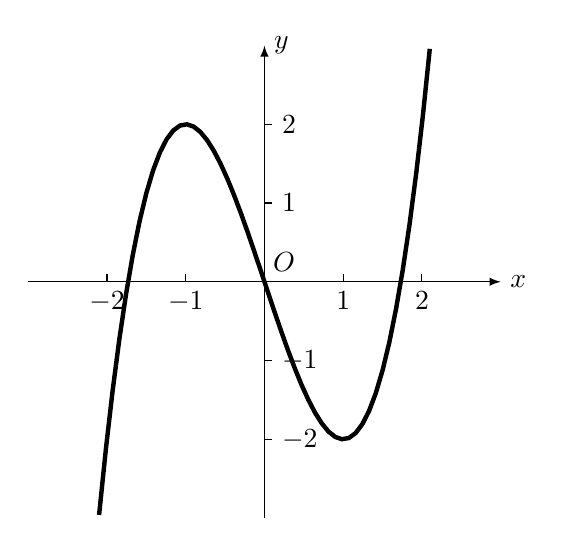
\begin{tikzpicture}[>=latex, scale=1]
        \draw[->] (-3,0)--(3,0)node[right]{$x$};
      \draw[->] (0,-3)--(0,3)node[right]{$y$};  
      \foreach \x in {-1,1,-2,2}
      {
          \draw (\x,0)node[below]{$\x$}--(\x,.1);
          \draw (0,\x)--(.1,\x)node[right]{$\x$};
      }
      \draw [domain=-2.1:2.1, samples=50, ultra thick] plot(\x, {\x*(\x*\x-3)});
    \node at (.25,.25){$O$};
    \end{tikzpicture}    
